\chapter{Diabetic retinopathy and its detection}\label{chapter3}
\section{The disease} \label{sec:disease}
Diabetic retinopathy is a common complication of diabetes, caused by high blood sugar levels damaging the blood vessels and nerve tissue of the retina. 

The earliest anatomical changes linked to the disease are the narrowing of the retinal arteries and the dysfunction of neurons of the inner retina. As the disease progresses damage may reach the outer retina, provoking subtle visual dysfunction, and weaken the blood-retinal barrier, that protects the retina from many substances present in blood, as immune cells or toxins.

In the later stages of the disease, the basement membrane of the retinal blood vessels thickens and the capillaries degenerate. This leads to a progressive ischemia of the tissues, which leads to degeneration of the neurons and glial cells of the retina. Narrower capillaries are prone to the appearance of microaneurysms, which may cause swelling or leak of them. 

Diabetic retinopathy is comorbid with macular edema, caused by the deposition of fluid and protein under the macula of the eye, causing it to thicken and swell.

\begin{figure}
    \centering
    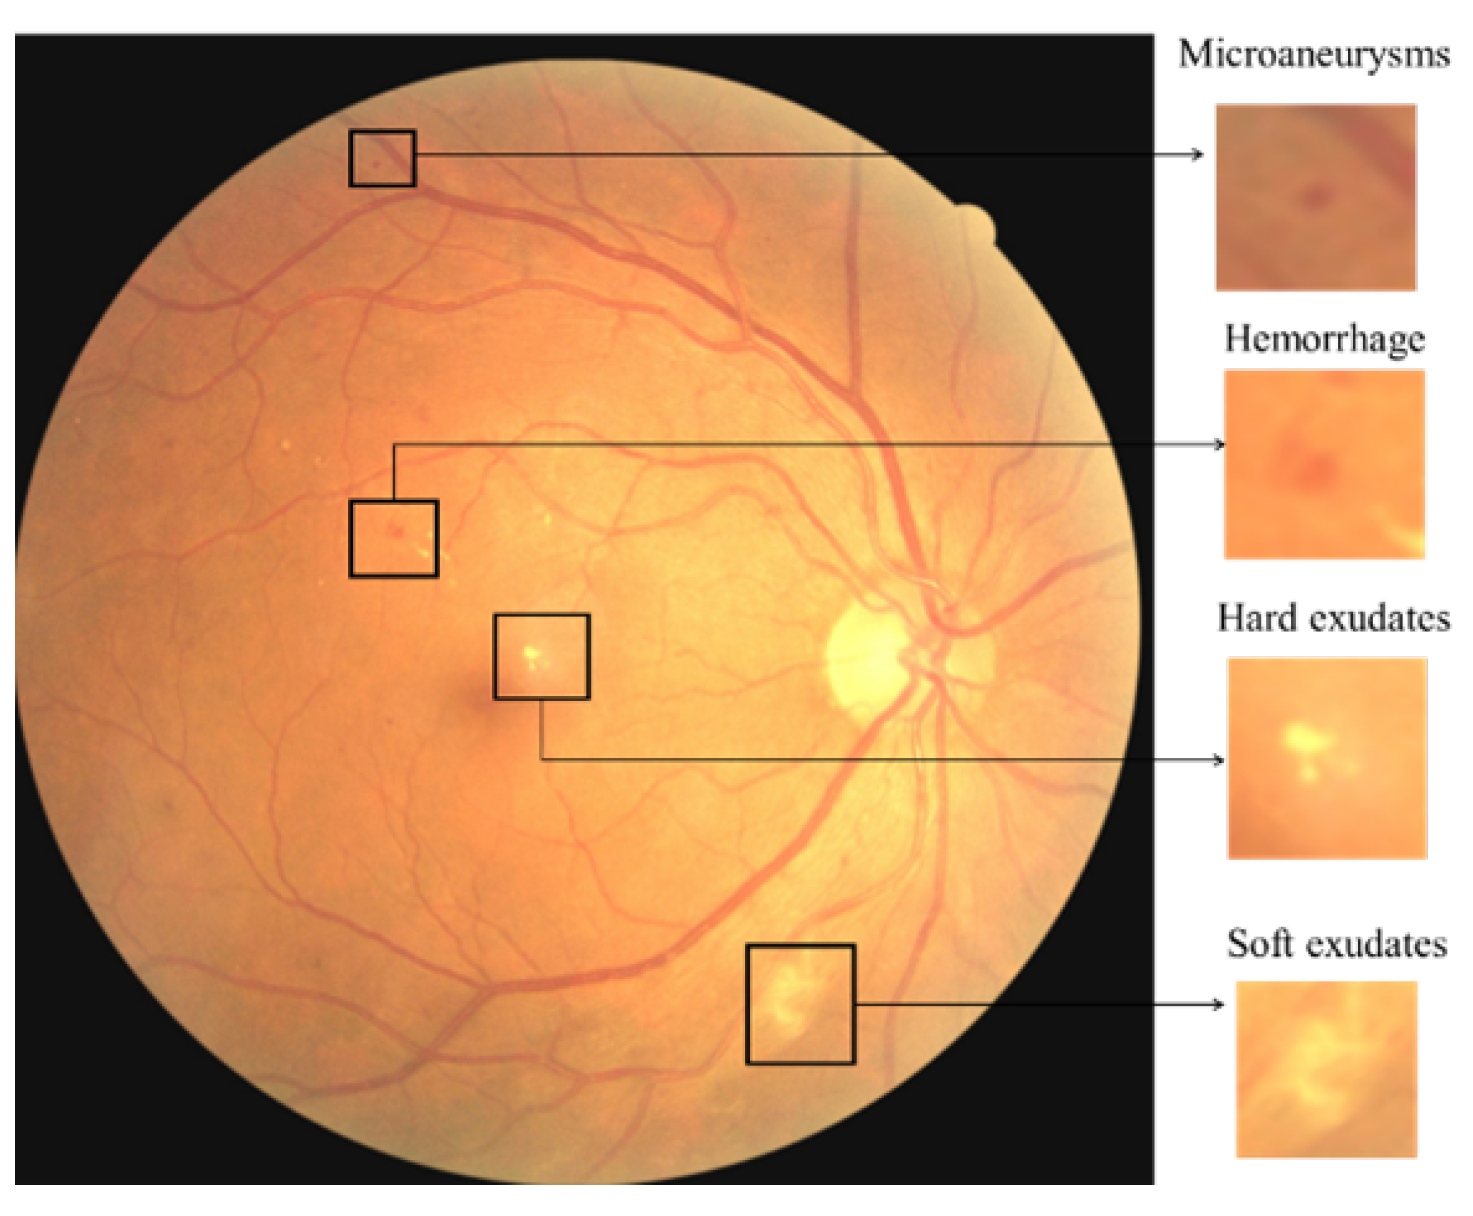
\includegraphics[width=\textwidth]{figures/chapter3/lesions.png}
    \caption{Example of lesions associated to diabetic retinopathy\cite{alyoubi2021images}}
    \label{fig:lesions}
\end{figure}

\subsection{Diagnosis and classification}
Since most symptoms develop in late stages of the disease, preventive retinal exams using \textit{opthalmoscopy} are key for detecting the disease on time. The classification of the disease is carried by a professional ophthalmologist who, following the guidelines of the American Academy of Ophthalmology, may classify the disease in one of five classes: no apparent retinopathy, mild, moderate or severe nonproliferative diabetic retinopathy (NPDR) or proliferative retinopathy (PDR).

People affected by mild NPDR have microaneurysms in the retina, but no other damage. Severe NPDR is diagnosed when more than 20 retinal hemorrhages are observed in each quadrant of the retina, blood vessels show a distinctive pattern of damage (venous beading) in at least two quadrants and there are clear intraretinal microvascular abnormalities. Moderate NDPR is an umbrella category that comprises cases more severe than mild NDPR but which don't meet all criteria to be considered severe. \Cref{fig:lesions} shows examples lesions indicating the presence of DR.

Proliferative DPR, the last stage of the disease, is characterized by the appearance of new very thin blood vessels (neovascularization) or blood leaking into the vitreous humor or between the vitreous membrane and retina. The \Cref{table:StagesDisease} summarizes the types of retinal lesions that can be found in the retina according to the stage of the disease in which the patient is found. 
\begin{table}[htbp]
\centering
\small
\begin{tabularx}{\textwidth}{|c|X|}
\hline
Class & Lesions Found \\ \hline \hline
No apparent retinopathy & No diabetic changes in the fundus and no microaneurysms \\ \hline
Mild retinopathy & Only microaneurysms are present \\ \hline
Moderate retinopathy & Microaneurysms associated with less than 20 hemorrhages in each of the 4 quadrants of the retina, presence of hard and soft exudates in only one quadrant \\ \hline
Severe retinopathy & Microaneurysms associated with more than 20 hemorrhages in all 4 quadrants or microvascular abnormalities in at least 2 quadrants and no signs of cardiovascular proliferation \\ \hline
Proliferative retinopathy & Formation of neovascularization and blood leaking into the vitreous humor (Haemovitreal) or between the vitreous membrane and retina (Pre-retinal) \\ \hline
\end{tabularx}
\caption{Lesions found depending on the disease stage \cite{diabetesSymptoms}. }
\label{table:StagesDisease}
\end{table}

It must be stressed that the diagnosis of diabetic retinopathy is a significant challenge even for specialist: a study involving the classification of over 6,000 images by two separate groups of clinicians found that grading agreed exactly on 69\% of cases and agreed within 1 level in 91\% of the cases \cite{gangaputra2013comparison}.

\section{Classical methods for computer-aided diagnosis}
The first methods to aid diagnosis of DR attempted to replicate the diagnostic guidelines for the disease, usually looking for morphological changes on blood vessels and the presence of lesions, especially microaneurysms and hemorrhages.

One of the most important breakthroughs in the fields came for the appearance of methods to segmentate blood vessels, which allows for the detection of vascular abnormalities. One of the first papers in the topic proposed the use of matched filter to detect piecewise linear segments of blood vessels. This was a challenging topic at the moment, since blood vessels usually have poor local contrast making general edge detection algorithms suboptimal \cite{chaudhuri1989detection}.

Apart from matched filtering, other unsupervised solutions were developed using tracking methods \cite{liu1993recursive, ali1999rapid}, multithreshold probing \cite{xiaoyi2003adaptive}, mathematical morphology \cite{zana2001segmentation} or a combination of centerlines and morphological reconstruction \cite{mendonca2006segmentation}. 

Supervised methods have also been used: for example, an influential paper repurposed a technique previously common in mammography analysis, line detection, to isolate blood vessels in the green channel of the retinal image \cite{ricci2007retinal}. Another very powerful method for blood vessels segmentation uses 2-D Gabor filters to enhance blood vessels and filter noise in a single operation \cite{soares2006retinal}.

The conclusions extracted from the analysis of the blood vessels can be reinforced by the detection of lesions, a significantly easier to approach problem. For example, the Indian Institute of Science created a model to classify three stages of DR (normal, moderate and nonproliferative diabetic retinopathy)\cite{verma2011detection}. To achieve this, they used a three steps approach:
\begin{enumerate}
    \item Detect blood vessels using segmentation techniques.
    \item Identify hemorrhages.
    \item Classification using Random Forests.
\end{enumerate}

This approach obtained 90\% of accuracy on normal cases and 87.5\%  on moderate and severe cases; very solid results, especially because they used a database of just 65 retinal images.

The main advantage of classical methods is that they require small datasets (usually just enough images to verify the performance of the algorithm under different conditions) and are generally interpretable, as they replicate diagnostic guidelines. However, some problems arise:
\begin{itemize}
    \item Usually, the translation of medical guidelines to computable properties is not straightforward. For example, measuring devascularization in this approach usually implies defining and computing properties as the fractal complexity of the blood vessels. The performance of the model is therefore highly dependent on the properties of the proxy properties chosen. 
    \item The solutions are tailored to the concrete disease. Usually most approaches cannot be reused to diagnose other (even similar) diseases. 
    \item The high complexity of the resulting algorithms implies that only a small fraction of the diagnostic guidelines can be properly evaluated. Information coming from the evaluation of some diagnostic guidelines is hard to reuse for the evaluation of others: for example, the interaction between lesions and vascular abnormalities is often lost in the process.
\end{itemize}

\section{Diagnosis based on deep learning models} \label{sec:diagnosis}
The application of deep learning models provoked a significant breakthrough in the field. Instead of trying to replicate the process followed by physicians when diagnosing a patient, these solutions used deep learning models (mainly convolutional neural networks) usually trained in a supervised fashion.

In a study of an algorithm for the disease in Retinal Fundus Images \cite{gulshan2016development}, the authors fine-tuned a CNN pretrained on ImageNet using 128.175 retinal images labeled by professional ophthalmologists. The model obtained over 90\% sensitivity and around 98\% specificity.  The authors worked with remarkably low resolution images, since they cropped the fundus images to the circular mask of the eye and rescaled them to have 299 pixels of diameter. 

A posterior study using an Inception-v3 architecture model, attained comparable results using four times less images for training \cite{sahlsten2019deep}. The authors found that models using very high resolutions (2095×2095) showed equivalent performance to an ensemble of models using 512×512 images, while the latter required just a fraction of time to train. 

A group of researchers from Pakistan and Vietnam \cite{qummar2019deep} got solid results for images with all degrees of the disease, overcoming previous limitations at detecting mild levels of affectation. The researchers proposed a model consisting on an ensemble of five different deep learning models: Resnet50, Inceptionv3, Xception, Dense121 and Dense169.

Deep learning models are data-hungry and usually require the manual labelling of data. To alleviate the problem, a group of researchers proposed an active learning approach that can generate labels for a set of unlabeled retinal images \cite{smailagic2020omedal}. The method uses the unlabeled examples that maximize the average distance to all training set examples, so it minimizes the required labels by selecting the unlabeled images that are most informative to the model as it trains. The model trains incrementally by using only the new set of labeled data and a subset of previously labeled data. 

An interesting variation of a CNN to provide enhanced interpretability avoided fully connected layers, using only convolutional and pooling layers in order to reduce the number of parameters and preserve locality of information \cite{wang2017diabetic}. By adding a regression activation map (RAM) after the global averaging pooling layer of the CNN it is possible to visualize the regions of diagnostic interest (\Cref{fig:interpreted_image}). While RAM is a technique that can be used in all CNNs, restricting the interaction between the different areas of the image makes sure that the resulting heatmap provides a precise assessment of the local significance of the region and has not been contaminated by the interaction between distant regions in the fully connected layers.

\begin{figure}[tb]
    \centering
    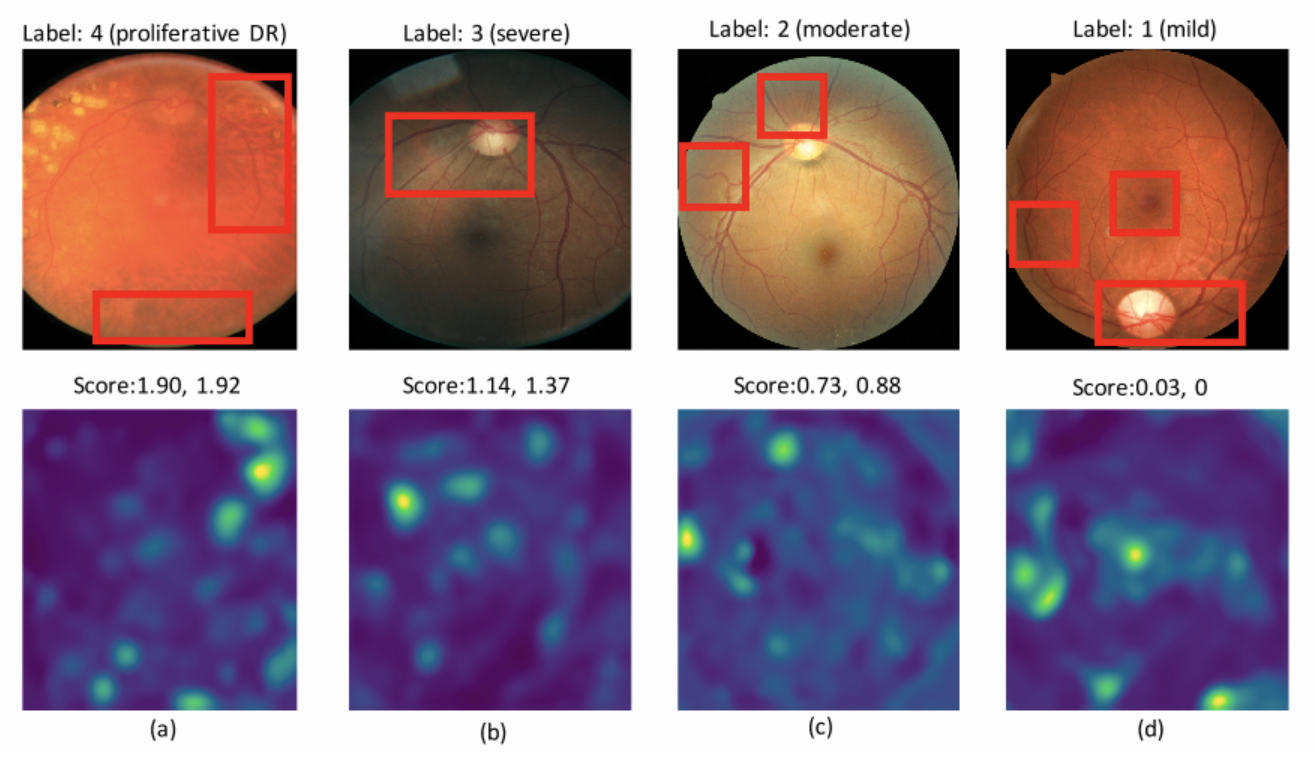
\includegraphics[width=\textwidth]{figures/chapter3/interpreted_image.png}
    \caption{By restricting the interaction between different areas of the image and including regression activation maps, it is possible to preserve the locality of the activations and highlight the main areas of diagnostic interest  \cite{wang2017diabetic}.}
    \label{fig:interpreted_image}
\end{figure}

Two researchers based in California \cite{gargeya2017automated} used custom convolutional neural networks to evaluate the degree of the disease. They later extracted the data-driven features and fed them to a tree-based classification model. In order to create a way to visualize the areas that were driving the classification (\Cref{fig:deep_features}), the authors implemented a convolutional layer at the end of the network, followed by an average pooling layer and a traditional softmax layer. With the information provided by the final layer a visualization heatmap is generated.

\begin{figure}[tbp]
    \centering
    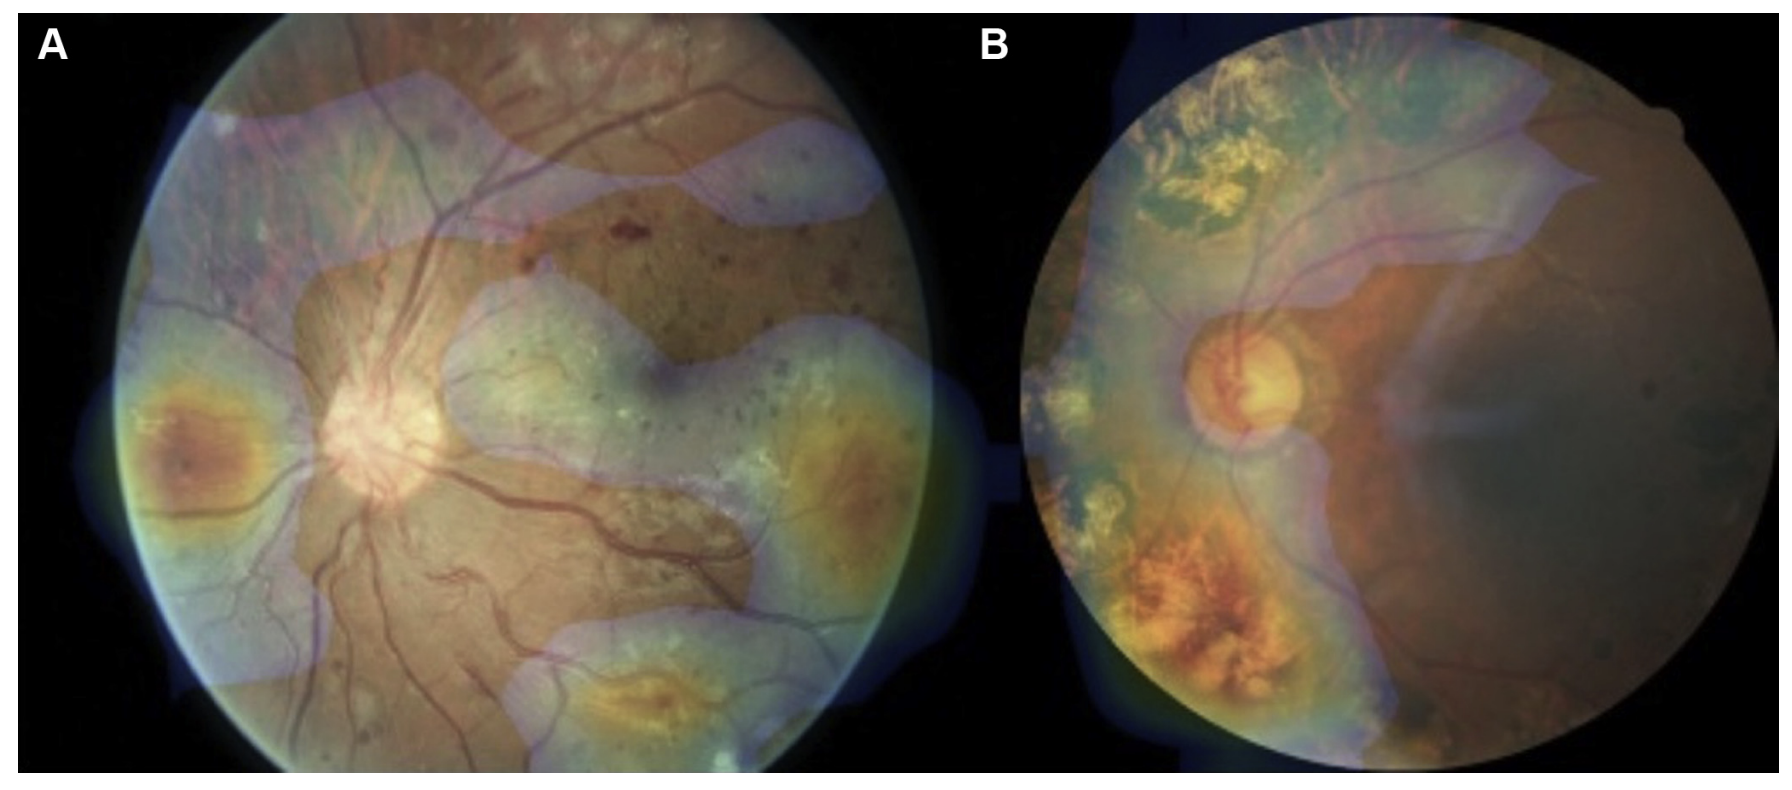
\includegraphics[width=\textwidth]{figures/chapter3/deep_features.png}
    \caption{Visualization of features to recognize areas of diagnostic interest \cite{gargeya2017automated}.}
    \label{fig:deep_features}
\end{figure}


An interesting source of models and ideas was the Kaggle Diabetic Retinopathy Detection sponsored by the California Healthcare Foundation \cite{diabeticretinopathydetection}. The challenge consisted on grading for DR images from the EyePacs dataset, with a training set of 35,000 images. The winning solution (presented by the team Min-Pooling in this competition report \cite{competitionReport}) used Fractional Max-Pooling \cite{graham2015fractional} to achieve a very solid performance. This technique introduced a stochastic variation of pooling that allows to reduce the size of the image by a non-integer fraction, choosing which regions are pooled randomly. All top-performing approaches used one or more CNNs in some cases combined with other techniques (such as random forests) to mix the information extracted from both eyes.

The correlation between DR and other diseases may be used to improve DR grading. Using the correlation between DR and diabetic macular edema (DME), it is possible to diagnose both diseases at the same time. One of the papers exploiting this idea  extracts features of the image using a backbone CNN and applies two attention blocks for every disease(\Cref{fig:edema}) \cite{li2020canet}. The first attention block is used to extract the specific features for each disease and the second one includes the features about the other disease influencing diagnosis. 

\begin{figure}[tbp]
    \centering
    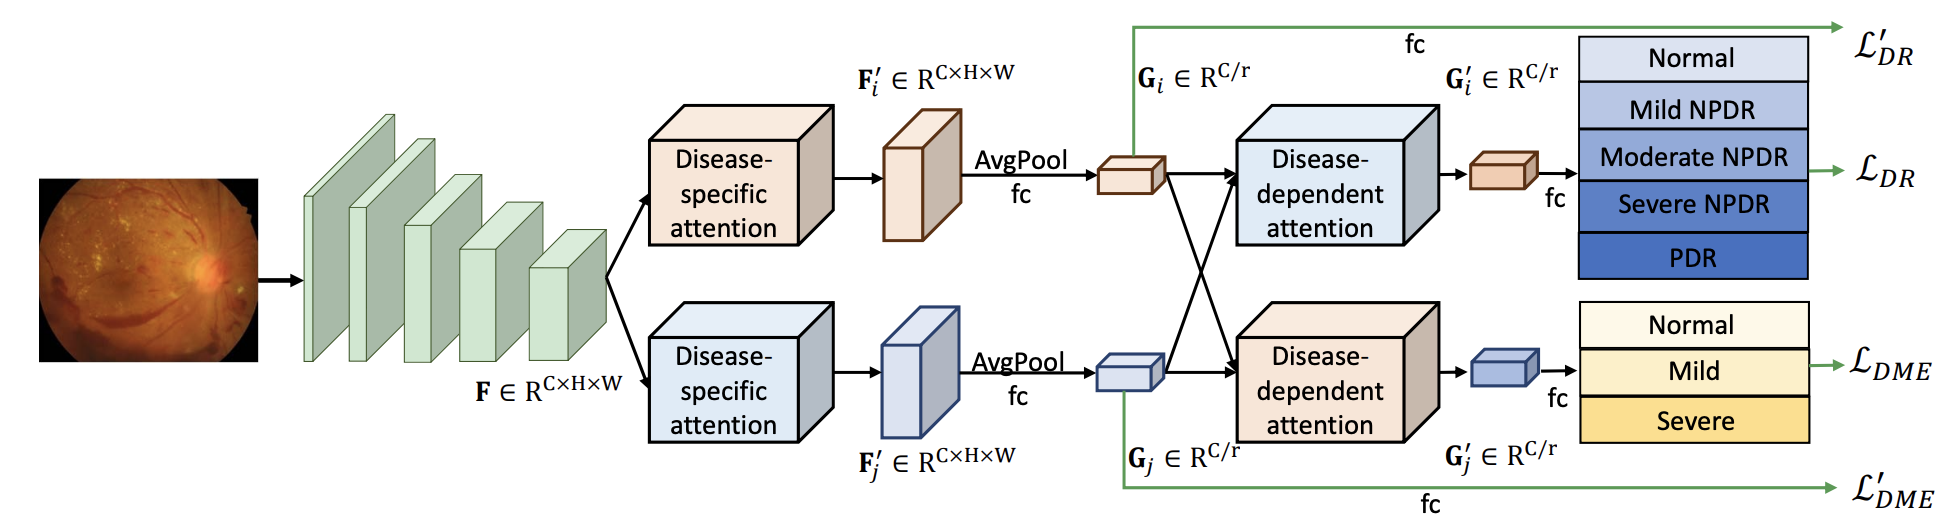
\includegraphics[width=\textwidth]{figures/chapter3/edema.png}
    \caption{Diagnosing DR and DME at the same time allows for the detection of disease specific and disease dependent features, achieving a better result than classifying both diseases independently \cite{li2020canet}.}
    \label{fig:edema}
\end{figure}

A \textit{zoom-in} technique has achieved state-of-the-art results on EyePACS and Messidor datasets \cite{wang2017zoom}. They used a complex architecture (\Cref{fig:zoom_in}) that attempts to mimic the process a clinician follows when examining an image: first, they skim the whole image and later they zoom-in on regions detected as problematic.

The model uses as a backbone an Inception-Resnet CNN to extract features of the images. A network generates attention maps for each levels of the disease. These attention maps are used to detect the areas with high response and a bounding box around them is drawn. The region corresponding to that area in the original image is then cropped and fed into a modified Inception CNN \cite{szegedy2016rethinking}.

This approach was able to detect up to 80\% of the areas marked as diagnostically significant by a professional.

\begin{figure}[tb]
    \centering
    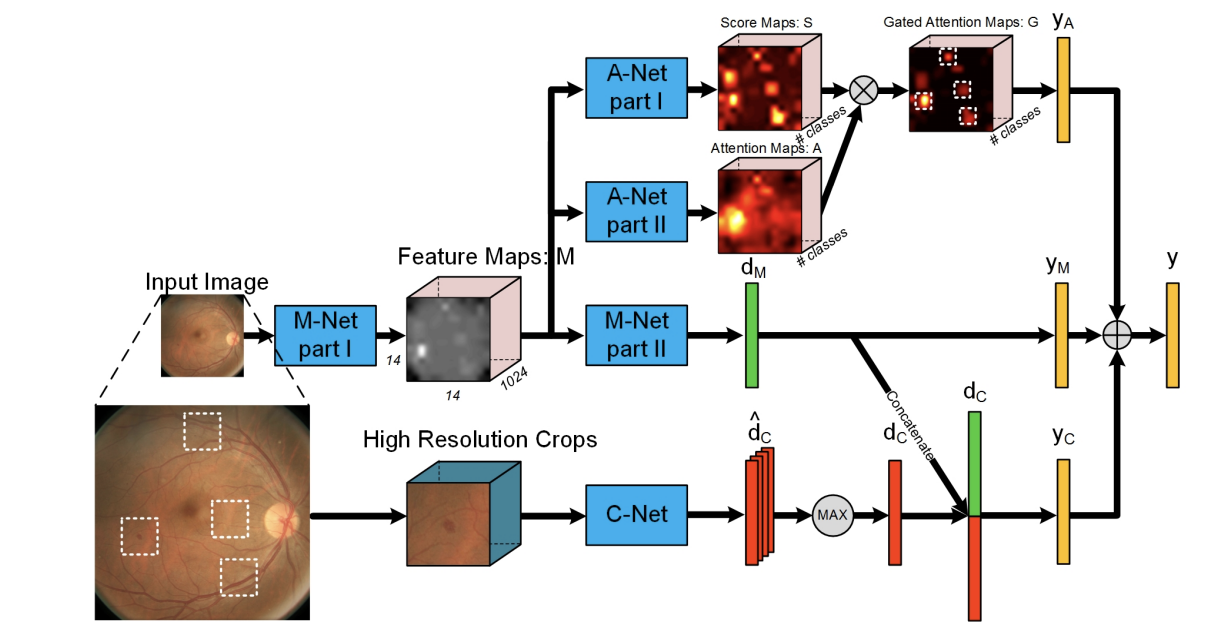
\includegraphics[width=\textwidth]{figures/chapter3/zoom_in.png}
    \caption{By combining a CNN with an attention mechanism, high activity areas can be localized. These areas can then be cropped from the original image, so a high resolution version of them is studied, simulating a \textit{zoom-in}\cite{wang2017zoom}.}
    \label{fig:zoom_in}
\end{figure}

Recent approaches to the problem of DR grading have experimented with the use of vision transformers instead of CNNs. A review comparing the performance of a CNN (Resnet50) and a vision transformer (DeiT-S) for different medical image classification problems (including DR) showed that CNN performs better than transformers when trained from scratch, perform equally when pretrained on ImageNet and are outperformed by transformers pretrained using self-supervision (DINO)\cite{matsoukas2021time}. The authors conclude that transformers can reliably replace CNN on medical image problems and stress the additional interpretability properties gained by using them. However, it must be noted that the Resnet50 model the researchers evaluated had been dominated by then by other architectures as EfficientNet.

Vision transformer (ViT) have two main drawbacks when applied to medical image classification: in first place, it is extremely data hungry which is a problem because medical images are notoriously hard to collect and label. In second place, the restriction to a single classification token may be excessively restricting. A group of researchers tried to overcome these limitations by adding an extra multiple-instance learning head to ViT, that creates a prediction using all the tokens but the class one  \cite{suang2021milvt}.

Another interesting transformer approach achieved state-of-the-art results with a lesion-aware model, that grades DR and discovers lesions simultaneously \cite{sun2021lesion-aware}. The model uses a pixel-based encoder and a lesion-based decoder to generate the input for the DR grading (\Cref{fig:lesion_encoder}). The ability of the encoder to adapt to different artifacts on pixels (like under or overexposure) results on an excellent performance discovering lesions.

\begin{figure}[tb]
    \centering
    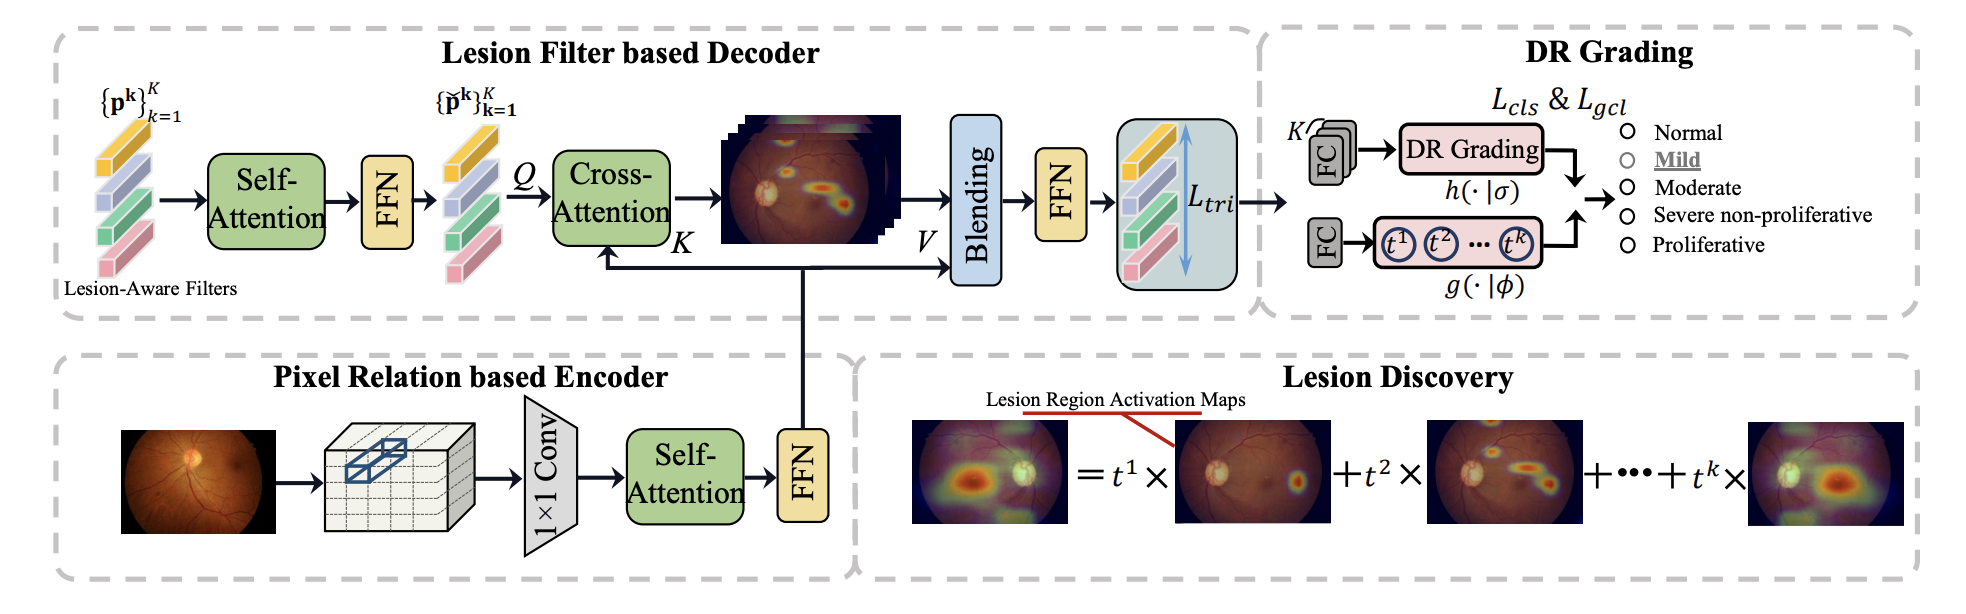
\includegraphics[width=\textwidth]{figures/chapter3/lesion_aware.png}
    \caption{Modeling the discovery of lesions as an encoder-decoder problem: the encoder identifies the relationship between pixels and the decoder detects lesions \cite{sun2021lesion-aware}.}
    \label{fig:lesion_encoder}
\end{figure}

The previous lines should serve to depict that the problem of diagnosing DR has been thoroughly studied, and significant progress has been made. Two families of deep learning model dominate the field: models using CNN as efficient feature extractors and other mechanisms, as attention layers, to provide better accuracy or interpretability on one hand and heavily customized transformers on the other hand. Out-of-the-box general purpose vision transformers usually have mediocre performance when applied to medical problems, but well-thought architectures appropriately trained can display unparalleled performance. 